\section{Background}
Understanding the intrinsic variability within the model is necessary when designing sets of experiments to ensure that the sample obtained is representative of generalized behavior.
Previous studies using the DeltaRCM methodology have run experiments in triplicate \cite{Liang2016a, Lauzon2018, Lauzon2019} as well as in sets of five \cite{Liang2016} to capture representative behavior under a given set of model conditions.
The underlying variability between model runs however, is not reported in these papers and remains an unknown (at the time of writing). 

\section{Model Runs}
\label{sec:standard_model_runs}
An ensemble of 30 model runs with different random seeds is generated.
These runs are at ``field-scale" using parameters similar to those from previous studies \cite{Liang2016, Liang2016a}.
The partial YAML file below provides information about the parameters used.\\

\noindent \texttt{YAML} configuration file: \vspace{-6pt}
\begin{boxedverbatim}
ensemble: 30
parallel: 3
Length: 7500
Width: 15000
timesteps: 5000
L0_meters: 150.0
N0_meters: 250.0
h0: 5.0
dx: 50
Np_water: 2000
Np_sed: 2000
save_dt: 250000
\end{boxedverbatim}

\section{Results}

Final topographies of all 30 deltas suggest that the overall shape and scale of these systems is similar (Figure \ref{fig:final_topos}). 
To quantify individual model behavior, land and channel maps are created by thresholding elevation and velocity data respectively.
Land is defined in locations where the elevation is at or above 0 m, and channels are pixels with velocity values in excess of 0.3 m/s (the threshold to mobilize sediment). 
Both of these thresholded arrays are bounded by a shoreline which is detected using morphological operators in a method similar to \citet{Geleynse2012}.
The method and its accuracy are not of primary interest here, but rather the differences between measurements from individual model runs. 

\begin{sidewaysfigure}[!htbp]
	\makebox[\textwidth][c]{
	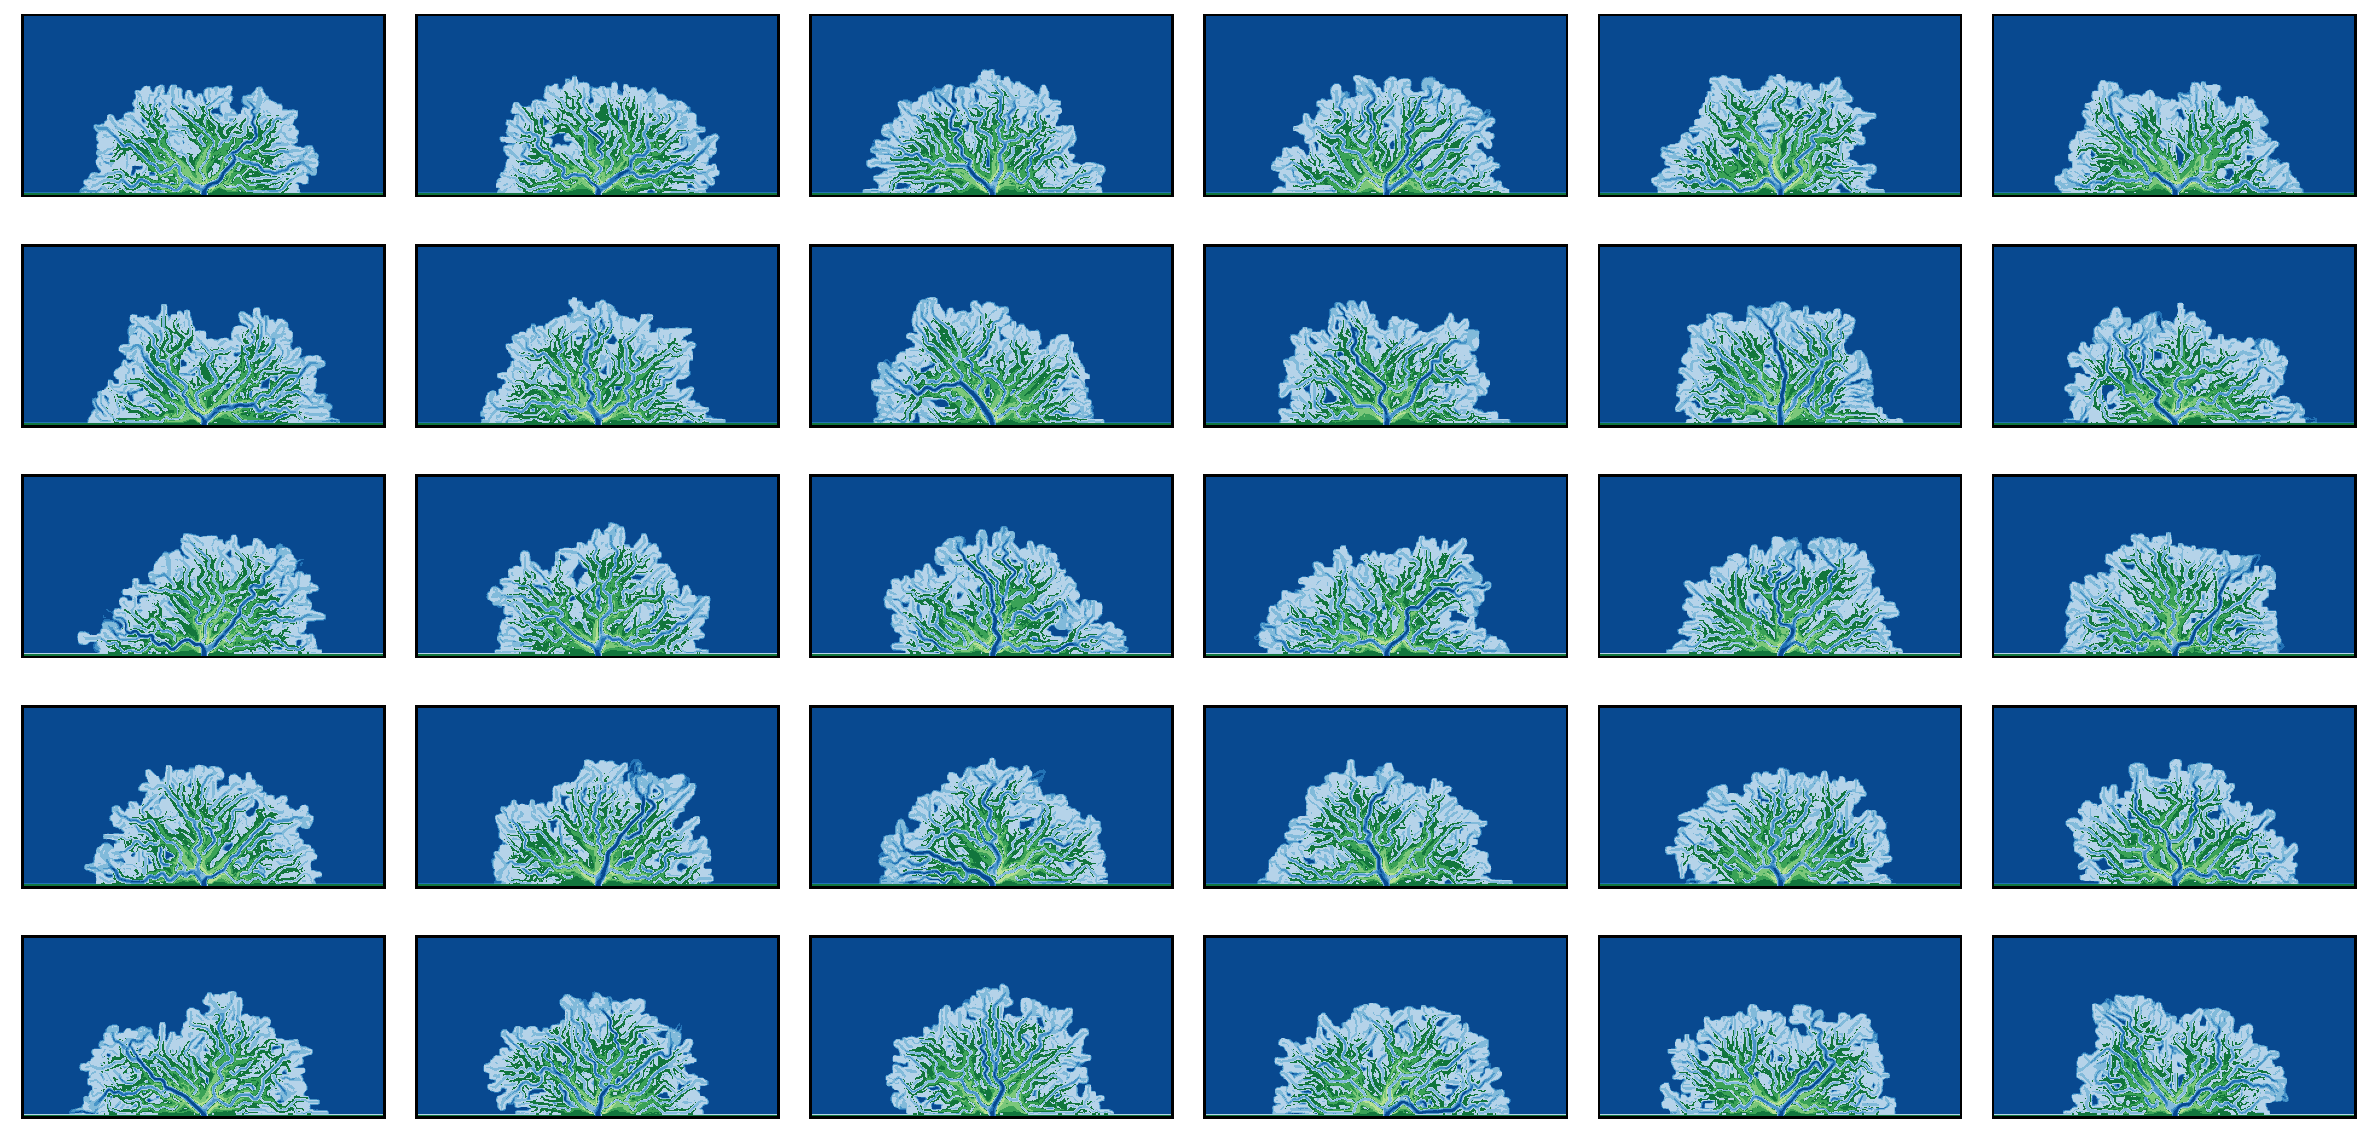
\includegraphics[width=\textwidth]{ModelVariability/figs/final_topos.pdf}
	}	
	\caption{Final topographies for the 30 ensemble runs.}
	\label{fig:final_topos}
\end{sidewaysfigure}

The three metrics measured are the land area, channel area, and fraction of land area that is channelized (channel fraction, Figure \ref{fig:surface_metrics}). 
Plots show individual replicate results in light gray, the ensemble mean in orange, and a blue envelope depicting the area within 1 standard deviation of the mean. 
Qualitatively there appears to be a fair amount of spread in these results.

\begin{sidewaysfigure}[!htbp]
	\makebox[\textwidth][c]{
	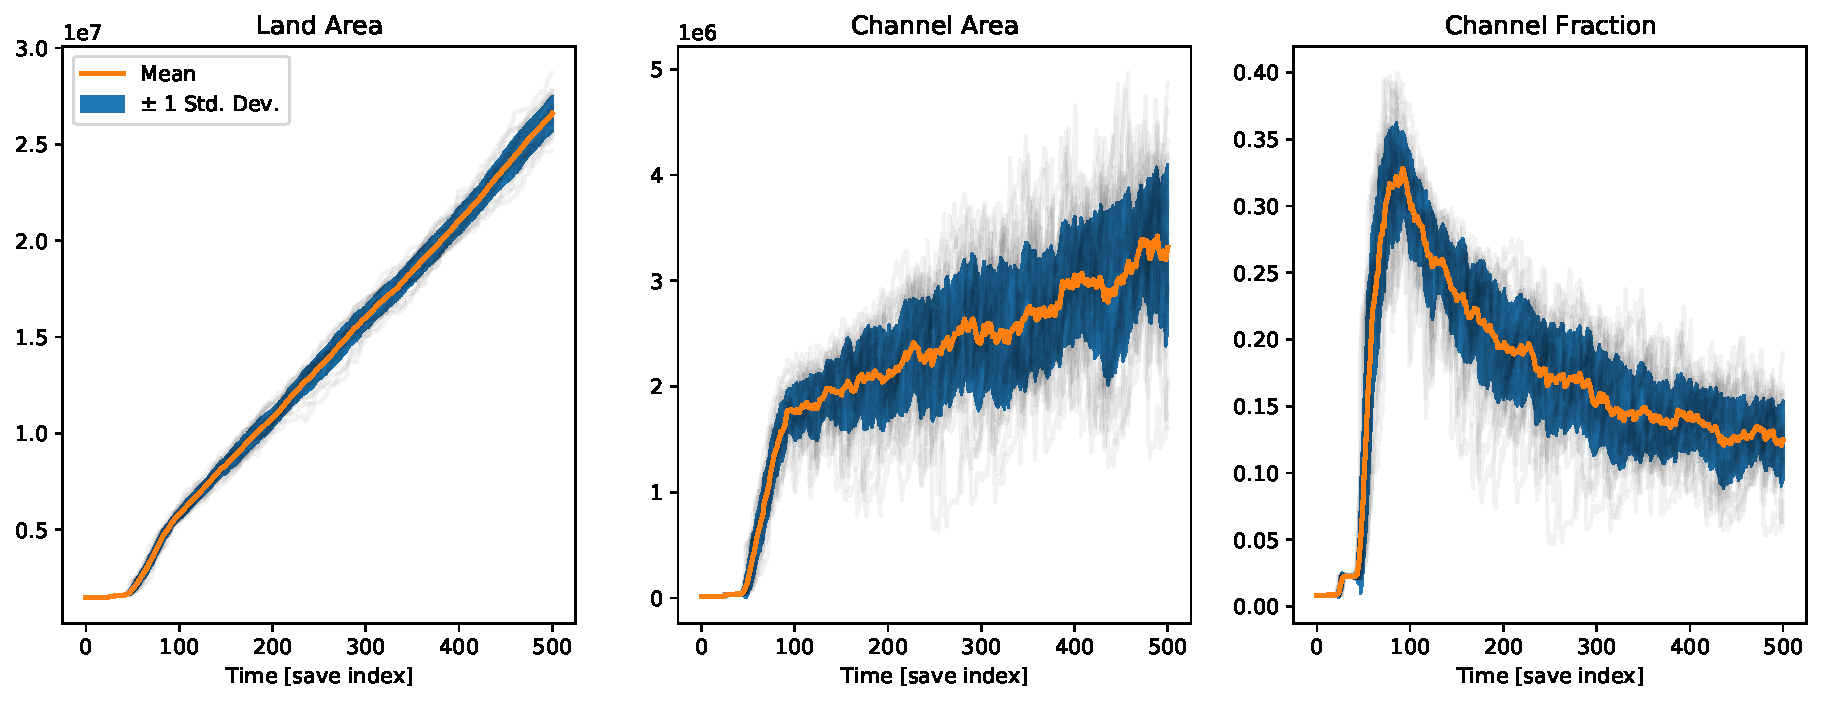
\includegraphics[width=\textwidth]{ModelVariability/figs/SurfaceTimeseries.pdf}
	}	
	\caption{Timeseries of 3 surface metrics: land area (left), channel area (center), and channel fraction, or the ratio of channel area to land area (right).}
	\label{fig:surface_metrics}
\end{sidewaysfigure}

To quantify this variability, a Monte Carlo approach is employed to estimate the probability of having a representative sample when using a smaller (less than 30) number of models.
The Monte Carlo method used works in the following way; to determine how representative a subset of $n$ models is, a random group of $n$ models from the full ensemble of 30 is chosen.
Next, a random point in time, $t_r$ is picked, and the land area, channel area, and channel fraction of the $n$ models is queried at time $t_r$, and a single average value for each metric is computed.
This average value is compared to the envelope plus/minus 1 standard deviation of the full ensemble mean (Figure \ref{fig:surface_metrics}), if the average value falls within the envelope, the Monte Carlo draw is deemed to be representative of the broader set.
The sampling process is repeated 1,000 times for each subset of $n$ models that is tested.
$n$ values between 1 and 10 are trialed as a reasonable range which includes the values of 3 and 5 used in previous studies.

For all three surface metrics evaluated, subsets of 3 or more models manage to fall within the `acceptable' envelope 90\% of the time or more. 
By the time the subset contains 7 models, this value has increased to 99\% (Table \ref{tab:tables}).
At 10 models, all three tables show nearly all draws fall within the envelope, suggesting that at least for these ``regular" or ``pseudo-default" parameters, no more than 10 models are needed to obtain a representative sample of model behavior for a given configuration.
Even subsets of fewer than 10 models are very likely to be representative of average behavior, anything above 3 appears to be a reasonable choice of replicates to use.

\begin{figure}[!htbp]
	\makebox[\textwidth][c]{
	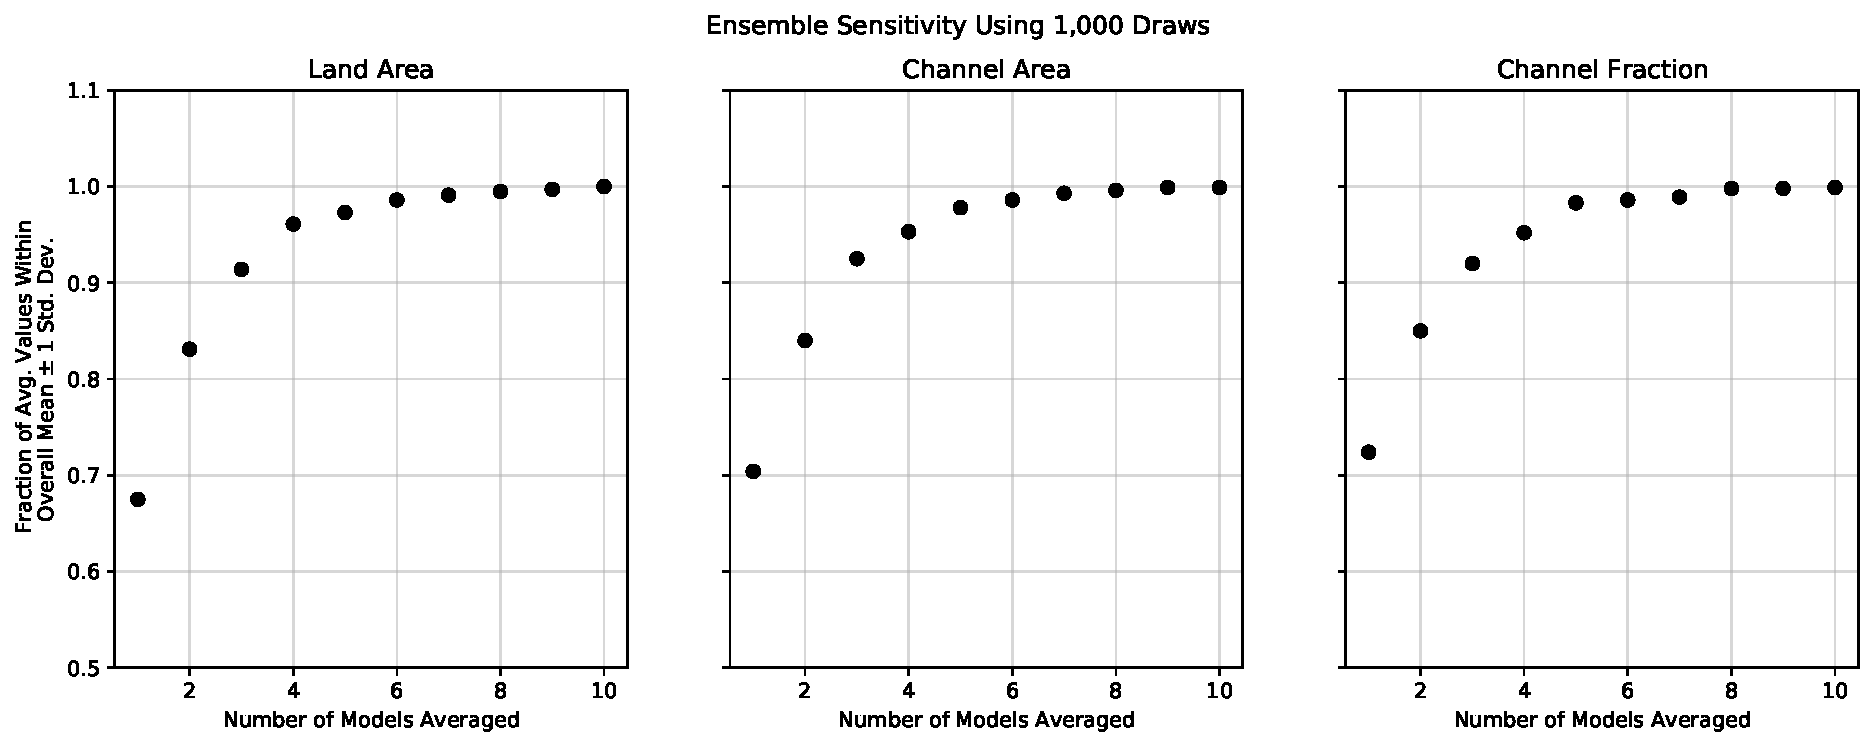
\includegraphics[width=\textwidth]{ModelVariability/figs/EnsembleSensitivity.pdf}
	}	
	\caption{Results of the sensitivity analysis for each of the surface metrics. Number of models in the Monte Carlo sampling along the x-axis and the fraction of average metric results within 1 standard deviation of the full dataset is on the y-axis.}
	\label{fig:MC_results}
\end{figure}

\begin{table}[!ht]
\begin{small}
\begin{tabular}{lcr}
\begin{minipage}[c]{0.3\linewidth}
\centering
\begin{tabular}{| l | r |}
\hline
\# Models & Fraction in Envelope \\
\hline
\hline
\csvreader[no head, late after line=\\\hline]
   {ModelVariability/tables/landsensitivity.csv}{}{\csvcoli & \csvcolii}
\end{tabular}
\label{tab:land}
\end{minipage}
&
\begin{minipage}[c]{0.3\linewidth}
\centering
\begin{tabular}{| l | r |}
\hline
\# Models & Fraction in Envelope \\
\hline
\hline
\csvreader[no head, late after line=\\\hline]
   {ModelVariability/tables/channelsensitivity.csv}{}{\csvcoli & \csvcolii}
\end{tabular}
\label{tab:land}
\end{minipage}
&
\begin{minipage}[c]{0.3\linewidth}
\centering
\begin{tabular}{| l | r |}
\hline
\# Models & Fraction in Envelope \\
\hline
\hline
\csvreader[no head, late after line=\\\hline]
   {ModelVariability/tables/fracsensitivity.csv}{}{\csvcoli & \csvcolii}
\end{tabular}
\label{tab:land}
\end{minipage}
\end{tabular}
\caption{Data from Figure \ref{fig:MC_results} presented in tabular form with the land area sensitivity on the left, channel area in the middle, and channel fraction on the right.}
\label{tab:tables}
\end{small}
\end{table}


\section{Conclusions}
While this is far from the most rigorous evaluation of intrinsic variability within the \textit{pyDeltaRCM} model, these results suggest that a minimum of 3 models should be run to characterize behavior representative of the domain and parameters. 
These results focus on just a few surface metrics, further tests should be conducted on the dynamics of the system as well as the stratigraphy produced, however given the number of studies previously conducted using 3 or 5 replicates, it is likely that unpublished sensitivity studies back up the findings reported here.

\clearpage
\bibliographystyle{plainnat}
\bibliography{bib/bib}